\documentclass[a4paper,10pt,uplatex,dvipdfmx]{jsarticle}


% 数式
\usepackage{amsmath,amsfonts}
\usepackage{bm}
% 画像
\usepackage[dvipdfmx]{graphicx}
\usepackage{here}
% プログラム
\usepackage{color}
\usepackage{listings,jlisting}

\title{画像・映像情報処理\\ \huge 第一回実習レポート}
\author{学籍番号:201811411\\ 所属:情報学群情報メディア創成学類\\ 氏名:加藤虎之介}
\date{\today}

\lstset{
 language={C},%言語の指定
%  backgroundcolor={\color[gray]{.85}},%背景色と透過度
 basicstyle={\ttfamily},%書体の指定
 identifierstyle={\small},%
 commentstyle={\small\itshape\color[rgb]{0,0.5,0}},%注釈の書体
 keywordstyle={\small\bfseries\color[rgb]{1,0,0}},%キーワード(int, ifなど)の書体指定
 ndkeywordstyle={\small},%
 stringstyle={\small\ttfamily},%文字列
 frame={tb},%枠縁(leftline,topline,bottomline,lines,trBL,shadowbox, single)
 breaklines=true,%折り返し(自動改行)
 breakindent = 10pt,  %自動改行後のインデント量(デフォルトでは20[pt])	
 columns=[l]{fullflexible},%
 numbers=left,%行番号表示
 xrightmargin=0zw,%
 xleftmargin=3zw,%
 numberstyle={\scriptsize},%行番号の書体指定
 stepnumber=1,
 numbersep=1zw,%
 lineskip=-0.5ex%
}
\renewcommand{\lstlistingname}{Code} % キャプション名の指定

\begin{document}
\maketitle
\section{課題1}
\subsection{平均値フィルタ}
\subsubsection{プログラム}
\lstinputlisting[caption = avg\_filter.c]{../src/avg_filter.c}

\subsubsection{実験結果}
\begin{itemize}
  \item $3\times3$の平均値フィルタをかけた結果
    \begin{figure}[H]
      \centering
      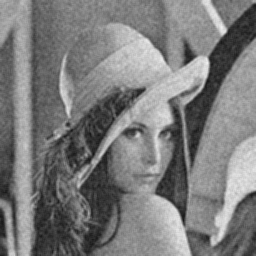
\includegraphics[width=5cm]{../src/img/output_avg3x3.png}
      \caption{$3\times3$の平均値フィルタ}
    \end{figure}
  \item $5\times5$の平均値フィルタをかけた結果
    \begin{figure}[H]
      \centering
      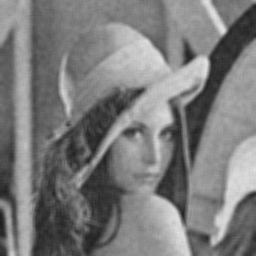
\includegraphics[width=5cm]{../src/img/output_avg5x5.png}
      \caption{$5\times5$の平均値フィルタ}
    \end{figure}
  \item $7\times7$の平均値フィルタをかけた結果
    \begin{figure}[H]
      \centering
      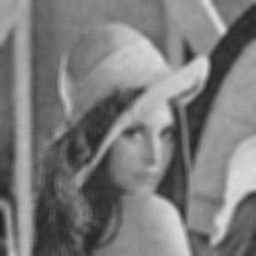
\includegraphics[width=5cm]{../src/img/output_avg7x7.png}
      \caption{$7\times7$の平均値フィルタ}
    \end{figure}
\end{itemize}

\subsubsection{実験結果に対する考察}
フィルタサイズを大きくするほど、雑音がよく除去されるが、エッジが滑らかになりボヤけた画像になった。

\subsection{メディアンフィルタ}
\subsubsection{プログラム}
\lstinputlisting[caption = median\_filter.c]{../src/median_filter.c}

\subsubsection{実験結果}
\begin{itemize}
  \item $3\times3$のメディアンフィルタをかけた結果
    \begin{figure}[H]
      \centering
      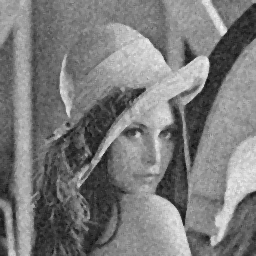
\includegraphics[width=5cm]{../src/img/output_median3x3.png}
      \caption{$3\times3$のメディアンフィルタ}
    \end{figure} 
  \item $5\times5$のメディアンフィルタをかけた結果
    \begin{figure}[H]
      \centering
      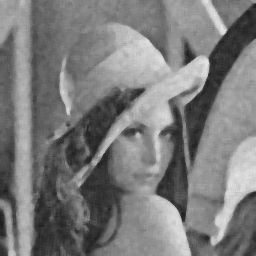
\includegraphics[width=5cm]{../src/img/output_median5x5.png}
      \caption{$5\times5$のメディアンフィルタ}
    \end{figure} 
  \item $7\times7$のメディアンフィルタをかけた結果
    \begin{figure}[H]
      \centering
      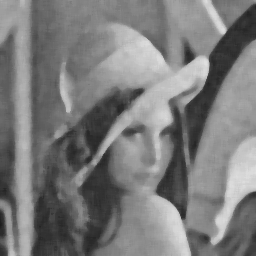
\includegraphics[width=5cm]{../src/img/output_median7x7.png}
      \caption{$7\times7$のメディアンフィルタ}
    \end{figure} 
\end{itemize}

\subsubsection{実験結果に対する考察}
フィルタサイズが大きくなる程、雑音の除去能力が高くなっている。また同一サイズの平均値フィルタに比べ、エッジの鋭さが保存されている。しかし、色の変化の滑らかさは失われ、色むらができている。

\section{課題2}
\subsection{ソーベルフィルタ}
\subsubsection{プログラム}
\lstinputlisting[caption = sobel\_filter.c]{../src/sobel_filter.c}

\subsubsection{実験結果}
\begin{itemize}
  \item $coefficient=0.20$のゾーベルフィルタをかけた結果
    \begin{figure}[H]
      \centering
      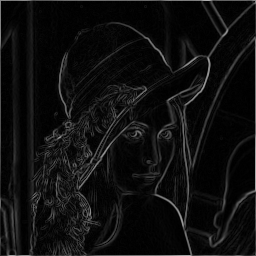
\includegraphics[width=5cm]{../src/img/output_sobel02.png}
      \caption{$coefficient=0.20$のゾーベルフィルタ}
    \end{figure} 
  \item $coefficient=0.50$のゾーベルフィルタをかけた結果
    \begin{figure}[H]
      \centering
      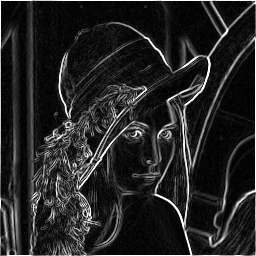
\includegraphics[width=5cm]{../src/img/output_sobel.png}
      \caption{$coefficient=0.50$のゾーベルフィルタ}
    \end{figure} 
  \item $coefficient=1.0$のゾーベルフィルタをかけた結果
    \begin{figure}[H]
      \centering
      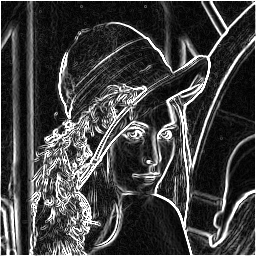
\includegraphics[width=5cm]{../src/img/output_sobel10.png}
      \caption{$coefficient=1.0$のゾーベルフィルタ}
    \end{figure} 
\end{itemize}

\subsubsection{実験結果に対する考察}
フィルタの出力値にかける係数(定数$coefficient$)の値を変化させると、出力される画像が変化した。係数を大きくすると検出されるエッジがより強調されるようになる。

\end{document}